
{construction}
Any quadratic equation in terms of $x,y$ of the form $ax^2+2bxy+cy^2+2dx+2ey+f=0$,can be written as
\begin{align}
    \vec{x}^T\vec{V}\vec{x}+2\vec{u}^T\vec{x}+f=0
%\label{eq:solutions/2/6/22/eq:2}
\\
    \text{where,}
    \vec{V}=\myvec{a&b\\b&c}\\
    \vec{u}=\myvec{d\\e}
\end{align}
The equation \eqref{eq:solutions/2/6/22/eq:1} represents two intersecting straight lines when
\begin{align}
    \mydet{\vec{V} & u\\u^T &f}=0\label{eq:solutions/2/6/22/eq:2}\\
    \mydet{\vec{V}}<0
\end{align}
{explanation}
From equation \eqref{eq:solutions/2/6/22/eq:1} we get
\begin{align}
    \vec{V}=\myvec{6&-\frac{1}{2}\\-\frac{1}{2}&-15}\\
    \vec{u}=\myvec{\frac{-11}{2}\\ \frac{31}{2}}\\
    f=-10
\end{align}
calculating the equation \eqref{eq:solutions/2/6/22/eq:2},we get
\begin{align}
    \myvec{6&-\frac{1}{2}&\frac{-11}{2}\\-\frac{1}{2}&-15&\frac{31}{2}\\\frac{-11}{2}&\frac{31}{2}&-10}\xleftrightarrow[]{R_3=R_3+R_2+R_1}\myvec{6&-\frac{1}{2}&\frac{-11}{2}\\-\frac{1}{2}&-15&\frac{31}{2}\\0&0&0}
\end{align}
Therefore the determinant $0$.And also the determinant of $\vec{V}$ is
\begin{align}
    \mydet{\vec{V}}&=\mydet{6&-\frac{1}{2}\\-\frac{1}{2}&-15}\\
    &=-90.25\\
    &<0
\end{align}
Therefore the given equation represents the equation of two straight lines which intersect.
{point of intersection}
The point of intersection of the straight lines is given by 
\begin{align}
    c&=-\vec{V}^{-1}\vec{u}
\end{align}
The inverse of $\vec{V}$ can be found by using rref of augmented matrix of the matrices $\vec{V}$ and $\vec{I}$
\begin{align}
    \myvec{6&-\frac{1}{2}&1&0\\-\frac{1}{2}&-15&0&1}\xleftrightarrow{R_2=12R_2+R_1}\myvec{6&-\frac{1}{2}&1&0\\0&-\frac{361}{2}&1&12}\\
    \myvec{6&-\frac{1}{2}&1&0\\0&1&-\frac{2}{361}&-\frac{24}{361}}\xleftrightarrow{R_1=R_1+\frac{R_2}{2}}\myvec{6&0&\frac{360}{361}&-\frac{12}{361}\\0&1&-\frac{2}{361}&-\frac{24}{361}}\\
    \vec{V}^{-1}=\myvec{\frac{60}{361}&-\frac{2}{361}\\-\frac{2}{361}&-\frac{24}{361}}\\
    c=-\myvec{\frac{60}{361}&-\frac{2}{361}\\-\frac{2}{361}&-\frac{24}{361}}\myvec{-\frac{11}{2}\\\frac{31}{2}}\\
    c=\myvec{1\\1}
\end{align}
Therefore the lines intersect at the point $\myvec{1\\1}$.
{eigenvectors}
The characteristic equation of the matrix $\vec{V}$ is
\begin{align}
    \mydet{\vec{V}-\lambda\vec{I}}&=0\\
    \mydet{6-\lambda&-\frac{1}{2}\\-\frac{1}{2}&-15-\lambda}&=0\\
    \lambda^2+9\lambda-90.25&=0
\end{align}
So the eigenvalues will be
\begin{align}
    \lambda_1=\frac{-1}{2}\brak{9+\sqrt{442}}\\
    \lambda_2=\frac{-1}{2}\brak{9-\sqrt{442}}
\end{align}
The eigen vectors will be in the nullspace of $\vec{V}-\lambda_1\vec{I}$ and $\vec{V}-\lambda_2\vec{I}$.The eigen vector corresponding to eigen value $\lambda_1$ will be
\begin{align}
    \vec{V}-\lambda_1\vec{I}=\myvec{6+\frac{1}{2}\brak{9+\sqrt{442}}&-\frac{1}{2}\\-\frac{1}{2}&-15+\frac{1}{2}\brak{9+\sqrt{442}}}\\
    =\myvec{\frac{1}{2}\brak{21+\sqrt{442}}&-\frac{1}{2}\\-\frac{1}{2}&\frac{1}{2}\brak{-21+\sqrt{442}}}\\
    \xleftrightarrow[]{R_2=\brak{21+\sqrt{442}}R_2+R_1}\myvec{\frac{1}{2}\brak{21+\sqrt{442}}&-\frac{1}{2}\\0&0}
\end{align}
The above reduced matrix has one free variable.Let it be $1$,then the eigen vector will be
\begin{align}
    {p_1}=\myvec{1\\21+\sqrt{442}}
\end{align}
normalizing $p_1$,we get
\begin{align}
    p_1=\frac{1}{\sqrt{884+42\sqrt{442}}}\myvec{1\\21+\sqrt{442}}
\end{align}
the eigen vector corresponding to eigen value $\lambda_2$ will be
\begin{align}
    \vec{V}-\lambda_1\vec{I}=\myvec{6+\frac{1}{2}\brak{9-\sqrt{442}}&-\frac{1}{2}\\-\frac{1}{2}&-15+\frac{1}{2}\brak{9-\sqrt{442}}}\\
    =\myvec{\frac{1}{2}\brak{21-\sqrt{442}}&-\frac{1}{2}\\-\frac{1}{2}&\frac{1}{2}\brak{-21-\sqrt{442}}}\\
    \xleftrightarrow[]{R_2=\brak{21-\sqrt{442}}R_2+R_1}\myvec{\frac{1}{2}\brak{21-\sqrt{442}}&-\frac{1}{2}\\0&0}
\end{align}
The above reduced matrix has one free variable.Let it be $1$,then the eigen vector will be
\begin{align}
    {p_2}=\myvec{1\\21-\sqrt{442}}
\end{align}
normalizing $p_2$,we get
\begin{align}
    p_2=\frac{1}{\sqrt{884-42\sqrt{442}}}\myvec{1\\21-\sqrt{442}}
\end{align}
So the transformation matrix will be 
\begin{align}
    \vec{P}=\myvec{p_1&p_2}=\myvec{\frac{1}{\sqrt{884+42\sqrt{442}}}&\frac{1}{\sqrt{884-42\sqrt{442}}}\\\frac{21+\sqrt{442}}{\sqrt{884+42\sqrt{442}}}&\frac{21-\sqrt{442}}{\sqrt{884-42\sqrt{442}}}}
\end{align}
{affine transformation}
Doing the affine transformation on given quadratic equation, we get pair to intersecting straight lines passing through origin.\par
Let the affine transformation be $\vec{x}=\vec{P}\vec{y}+c$.The transformation will be
\begin{align}
    \brak{\vec{P}\vec{y}+c}^T\vec{V}\brak{\vec{P}\vec{y}+c}+2\vec{u}^T\brak{\vec{P}\vec{y}+c}+f=0\\
\end{align}
    \begin{multline}
        \vec{y}^T\brak{\vec{P}^T\vec{V}\vec{P}}\vec{y}+2\brak{c^T\vec{V}+\vec{u}^T}\vec{P}\vec{y}\\
        +c^T\vec{V}c+2\vec{u}^Tc+f=0
\label{eq:solutions/2/6/22/eq:5}
    \end{multline}
\begin{figure}[t]
    \centering
    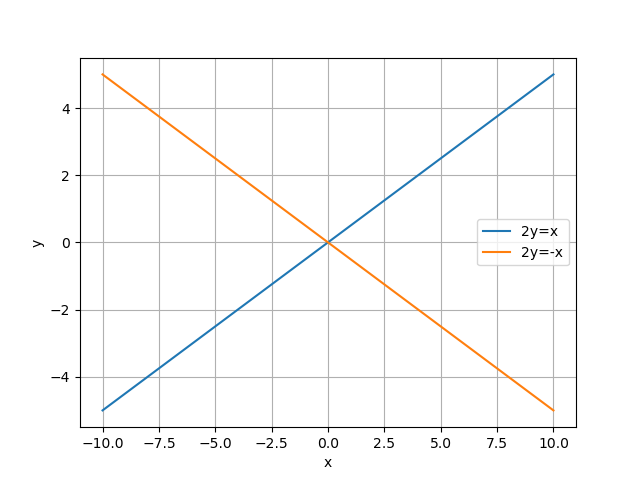
\includegraphics[width=\columnwidth]{./solutions/2/6/22/Fig1_a5.png}
    \caption{straight lines after affine transformation passing through origin}
    \label{eq:solutions/2/6/22/fig:1}
\end{figure}
if the point c is taken as the point of intersection of the two lines.
\begin{align}
    c^T\vec{V}c+2\vec{u}^Tc+f=0\\
    c^T\vec{V}+\vec{u}^T=0
\end{align}
So the affine transformation of the given lines will be
\begin{align}
    \vec{y}^T\brak{\vec{P}^T\vec{V}\vec{P}}\vec{y}=0\\
    \vec{y}^T\myvec{-1.5&0\\0&6}\vec{y}=0\\
    \brak{x-2y}\brak{x+2y}=0
\end{align}
Since the two lines are symmetric with respect to both $X-axis$ and $Y-axis$,the axes themselves are the bisectors of the transformed pair of lines.So the bisectors will be $x=0$ and $y=0$.
Matrix notation will be of the form
\begin{align}
    \vec{y}^T\myvec{0&0.5\\0.5&0}\vec{y}=0\\
    \vec{y}^T\vec{K}\vec{y}=0\\
    \vec{K}=\myvec{0&0.5\\0.5&0}
\end{align}
{bisectors}
Taking the inverse of the affine transformation of the equation $xy=0$,will give the angle bisectors.
\begin{align}
    \brak{\vec{P}^{-1}\vec{x}-\vec{P}^{-1}c}^T\vec{K}\brak{\vec{P}^{-1}\vec{x}-\vec{P}^{-1}c}=0\\
    \vec{x}^T\vec{P}\vec{K}\vec{P}^T\vec{x}-2c^T\vec{P}\vec{K}\vec{P}^T\vec{x}+c^T\vec{P}\vec{K}\vec{P}^Tc=0
\end{align}
Substituting the values we get
    \begin{multline}
        \vec{x}^T\myvec{\frac{1}{2\sqrt{442}}&\frac{21}{2\sqrt{442}}\\\frac{21}{2\sqrt{442}}&-\frac{1}{2\sqrt{442}}}\vec{x}\\
        -\myvec{\frac{22}{\sqrt{442}}&\frac{20}{\sqrt{442}}}\vec{x}+\frac{21}{\sqrt{442}}=0
    \end{multline}
    \begin{multline}
        \frac{x^2}{2\sqrt{442}}+\frac{21}{\sqrt{442}}xy-\frac{y^2}{2\sqrt{442}}\\
        -\frac{22x}{\sqrt{442}}-\frac{20y}{\sqrt{442}}+\frac{21}{\sqrt{442}}=0
    \end{multline}\\
\begin{align}
    x^2+42xy-y^2-44x-40y+42=0
\end{align}
Therefore the equation of bisectors of the given line in quadratic form is
\begin{align}
    \vec{x}^T\myvec{1&21\\21&-1}\vec{x}-\myvec{44&40}\vec{x}+42=0
\end{align}
\begin{figure}[t]
    \centering
    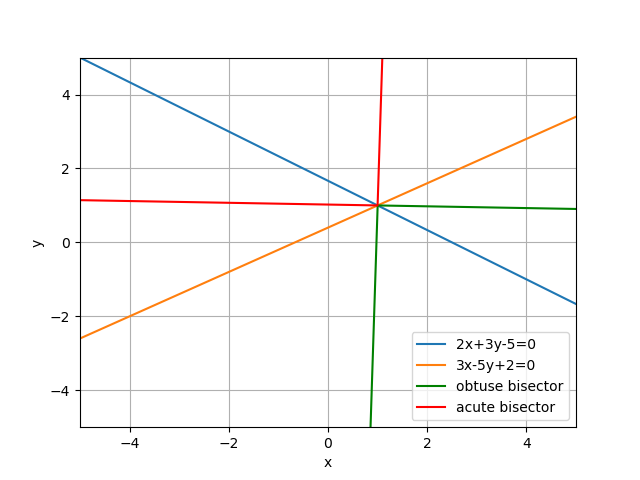
\includegraphics[width=\columnwidth]{./solutions/2/6/22/Fig2_a5.png}
    \caption{Par of straight lines and their angular bisectors}
    \label{eq:solutions/2/6/22/fig:my_label}
\end{figure}
